% ----------------------------------------------------------------
\documentclass[12pt,a4paper]{article}

\usepackage[british,UKenglish]{babel}  %% Language
\usepackage[a4paper, margin=1in]{geometry} %% margins
\usepackage{natbib} %% References
\usepackage[a4paper,bookmarks=true, colorlinks=false]{hyperref} % Links - must be last package

\usepackage{graphicx}
\usepackage[section]{placeins}
\graphicspath{ {images/} }


\usepackage{csquotes}
\usepackage{tikz}
\usepackage{gantt}
\usepackage{listings}

\begin{document}

\title{Parallelize Operations on a Durable Queue by Using Log Structured Storage with Memory Interleaving}%
\author{Avinash D'Silva \\ 15028534 \\ MSc in Cloud Computing}%
\date{\today}
\maketitle

\begin{abstract}
 In the recent years, Queues have emerged as the de-facto standard for various purposes such as asynchronous processing, buffering and load balancing. Queues primarily have two operations, enqueue and dequeue. These operations are parallel in theory but in practice when implemented as a durable queue, they tend to become more akin to an ACID compliant database system and hence loose their ability to perform operations in parallel. The durability of a queue cannot be compromised and yet at the same time, the need for performance is ever more increasing as queues have become the backbone of most distributed systems. This proposal will focus on Log Structured Storage along with Memory Interleaving and how a combination of these could make it possible for a queue to be durable as well as be able to perform parallel operations at the same time.
\end{abstract}

% TOC
\tableofcontents

\section{Introduction}

Queues are not a modern invention related to the field of Computer Science. They have existed well over the centuries. People queue up instinctively when there is a crowd for any given situation \citep{spieser2008stabilizing}. Queues, particularly in the field of Computer science, are known for their FIFO(First in First Out) data flow \citep{maclaren1969art}. Queues were initially used for simple well-known tasks such as enqueueing a print task on a printer, for breadth first search and have applications in graph theory. \\

 The structure of a queue very simple to understand and implement and queues in the recent years have become the backbone of distributed systems \citep{lamport1978time}. They are used for asynchronous processing, message passing, buffering and load balancing \citep{lu2011join}. 

 The size of data that most public facing applications have to deal with has been growing. There is ever more data from different IoT devices, Cell phones and Communication satellites and hence this age is called the Age of Big Data \citep{10333611920150101} \citep{lohr2012age}.\\
 
 
 The distributed systems have come under heavy load due to this growth in the size of data. One of the important part of a distributed system, the queues, are the most affected as these are the ones that carry and distribute the data throughout the system \citep{lamport1978time}. Queueing servers are becoming a bottleneck due to their fundamental shortcoming of not supporting parallel operations. The Figure \ref{fig:gull} shows how queues are implemented currently and shows how producers and consumers both use a single Write Ahead Log for durability. The Write Ahead Log only allows one operation at a time to be logged and hence queues aren't parallel due to this persistence layer.\\ 
 
 \begin{figure}[!htb]
 	\centering
 	\textbf{}\par\medskip
 	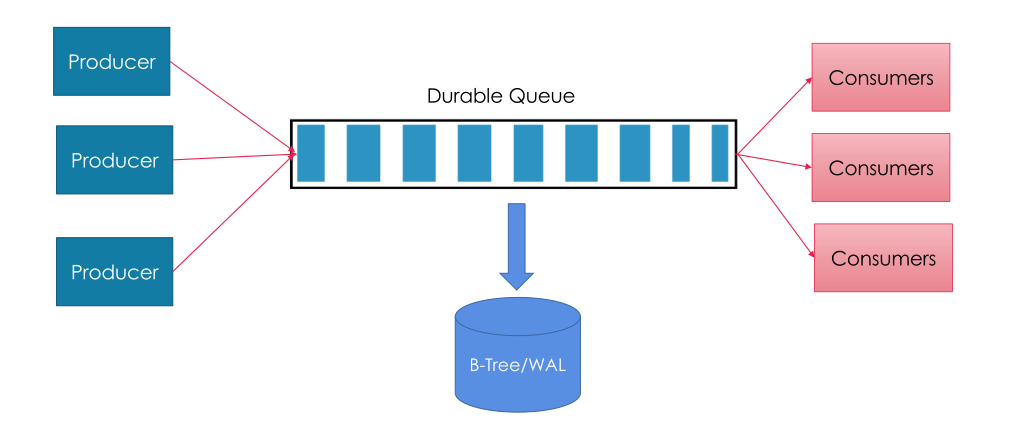
\includegraphics[scale=0.6]{1}
 	\caption{Overall architecture of the current queueing systems}
 	\label{fig:gull}
 \end{figure}
 
 

    
 Although queues are parallel in theory, they lose their parallel nature due to reliance on external disk-based storage structures such as B-Trees and WAL(Write Ahead Log) for durability. Queueing servers use various workarounds such as fanout queues and clustering as shown in Figure \ref{fig:gdulld} \citep{albrecht2013making}.\\

 
 
\begin{figure}[!htb]
   	\centering
   	\textbf{}\par\medskip
   	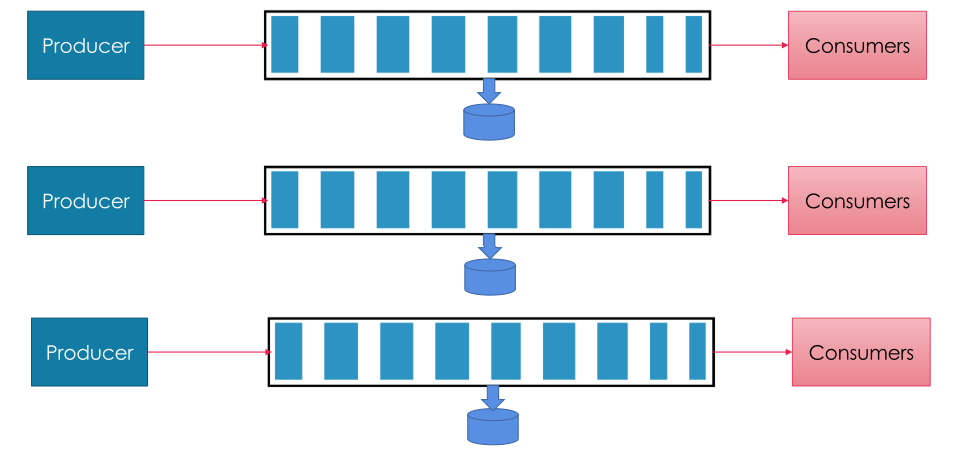
\includegraphics[scale=0.6]{2}
   	\caption{Achitecture of a clustered queueing systems}
   	\label{fig:gdulld}
\end{figure}
     
 
 The method of fanning out or clustering involves using multiple queues instead of a single queue to better handle the load. These multiple queues are abstracted as a single queue. One queueing server acts as a master while the rest act as slaves. These queues can be either mirror replicated or sharded \citep{albrecht2013making}. This type of setup is widely used in the industry today and almost all major queuing servers support the feature of clustering \citep{kermarrec2013xl}. But this doesn't solve the fundamental problem of durable queues not being parallel. This proposal describes the ways and means to parallelize operations on a durable queue using a combination of well-known technique of memory interleaving and Log Structured Storage.

 
\section{Literature Review}
\label{ric:litreview} % use labels to point to parts of your work

This proposal encompasses two primary techniques, Memory Interleaving and Log Structured Storage. The following sections will describe each of them, how they were used to solve similar problems and in what way are they relevant to this proposal.

\subsection{Distributed Computing}

	 Distributed computing as described by \citep{coulouris2005distributed} 
	 \enquote{is a field of computer science that studies distributed systems. A distributed system is a model in which components located on networked computers communicate and coordinate their actions by passing messages}
	 
	 Distributed computing is known as one of the ways to scale a computing system. The simplest example of a successful distributed system is the DNS(Domain Name System). Here DNS nodes act as servers which map a domain name to an IP address. The updates of these records are passed on from a server to another which is called as DNS propagation.\\
	 
	 Distributed system are used for solving problems that are too big for a single Computing node to solve. Multiple nodes are linked together so as to solve a single problem. The load is distributed across all of these nodes \citep{sukumar2007distributed} \citep{peleg2000distributed}. The link or connection between these nodes can either be continuous or it can connect as and when required.
	 Connection types can vary based on the protocol used. if a stateless protocol such as HTTP is used, then a continuous connection will be not be used \citep{berners1996hypertext} and if it is a stateful protocol then a continuous connection will be used. One of most used protocols in Distributed Computing is the Gossip Protocol \citep{kermarrec2007gossiping}. Queueing systems differ based on the connection type and are responsible how distributed systems are designed. If the connection between the queueing server and a compute node is stateless then the entire distributed system can be considered as a stateless system and stateless systems are the ones that scale the best \citep{gorton2003copyright}. 
	  
	  
\subsubsection{Tools for Distributed Computing}

Tools used in Distributed computing can differ based on the architecture used. if it is a tightly coupled stateful architecture then compute nodes would be directly connected to each other without a middleware such a queueing system but if it is a loosely coupled architecture, then the connection can be done via Map reduce environment or a careful configuration of task queues. Map-reduce can dynamically at internet scale \citep{costa2013internet}. It doesn't need configuration of pathways between the nodes nor any kind of ordering is required. Map reduce could be called automated queues.\\

Queues, on the other hand, require a lot of manual configuration. Queues include a lot of detail which Map reduce system users take it for granted such as the priority of data elements, expiration of data elements, defining retries and error queues \citep{mckenzie1994cranium}. Delivery Methods in queues also bring another layer of complexity. The delivery methods include "at most once", "at least once" and "exactly once" \citep{toshniwal2014storm}.


at most once delivery equals least reliability where the message can be delivered once or less than once. at least once delivery method ensures the message is delivered to at least one compute node. at least once delivery is currently the most used delivery mechanism \citep{toshniwal2014storm}. exactly once is to ensure no two compute nodes receive the same message. This method is difficult to implement and requires a lot of engineering effort \citep{amit2007guaranteed}.
	
\subsubsection{Queues in Distributed Computing}
Queues are heavily used in the field of distributed computing. They act as a glue between different computing instances. They are used for communication between two essentially disparate systems \citep{arroyo2006method}. if a system cannot communicate with each other due to differences in protocols, architecture or standards, a queue acts as a middleware between these systems. It allows heterogeneous systems to work together \citep{arroyo2006method}.\\

 
 \begin{figure}
 	\centering
 	\textbf{}\par\medskip
 	\includegraphics[scale=0.7]{3}
 	\caption{Achitecture of a distributed system connected with queues}
 	\label{fig:gdull03}
 \end{figure}

Another well-known use of queues is for the use of buffering, this method involves buffering the tasks on the queue and processing the tasks as and when the compute nodes are free. This could be an overnight job or a continuous job such as generating reports in the background. Queues can also be used to bring asynchronous nature to the distributed system. once a node puts a task on the queue, it can continue with its processing and some other node can pick up the job and process it.\\

As shown in Figure \ref{fig:gdull03} servers communicate with each other using queues, the communication is entirely asynchronous in nature. If server 1 pushes something on to the queue, then all other servers including itself can read from the queue. These servers may be of different architectures and may have been programmed in different languages, the queue becomes an abstraction layer for servers to communicate with each other\citep{shiang2008queuing}.


\subsubsection{Types of Queues used in Distributed Computing}
Although there is no standard classification of queues, They are classified by IronMQ, an Enterprise Queueing System in the manner the data is sent and received.

\begin{description}
	\item [Push Queue:] 
	 		Push Queues are queues wherein the queueing server pushes messages to the
	 		worker nodes. The rate at which the messages are sent can be configured.
	\item [Pull Queues:]
			 Pull Queues are queues wherein the workers pull messages from the queueing server. The rate at which the messages are pulled is decided by worker itself.
	
\end{description}

There could be a mix of both worlds implemented by an opensource job delegation server called Gearman wherein the queueing system switches from pull queue to push queue or vice-versa based on the workload.





\subsection{Log Structured Storage}

Log structured storage came as a new file system designed in 1988 and implemented in 1992 called the Log Structured File System \citep{rosenblum1992design}.\\

As shown in the figure \ref{fig:gdull04}, the older data resides as it is and is not overwritten, new data is simply appended to the end. The pointer to the new location is updated. If at all there is any during the write operation, the data pointer will simply point to the older revision. The writes are all asynchronous and this is the basis of a log structured system  \citep{rosenblum1992design}. 

 \begin{figure}
 	\centering
 	\textbf{}\par\medskip
 	\includegraphics[scale=0.8]{4}
 	\caption{Data inside a Log Structured System}
 	\label{fig:gdull04}
 \end{figure}

\subsubsection{Problem of File Corruption}
The problem with file systems or any kind of databases before Log Structured Storage was complex crash recovery procedures, and slow write speeds. File systems would rely heavily on error checking and would be complex to implement on a distributed environment \citep{swinehart1979wfs}
	
\subsubsection{Reliability gains and Cons}
Log Structured systems improved the reliability as it became very easy to recover from a crash just by moving the pointer to the previous location. The write speeds had increased as the system was asynchronous and an acknowledgement from the disk was no longer required. Any corruption from the hardware side could now easily be reverted by doing a simple log based undo operation \citep{reuter1980fast}.

\subsubsection{Derivates of Log Structured Storage}
Due to the data being never over written, they are used for time series databases or historical data access \citep{muth2000lham}. They are used in queues such as Apache Kafka which use log based storage that have multi cursor and "exactly once" delivery support\citep{kreps2011kafka} which is easily possible by a log based storage structure. Figure \ref{fig:gdull05} shows how messages are stored and segmented.  \\

 \begin{figure}
 	\centering
 	\textbf{}\par\medskip
 	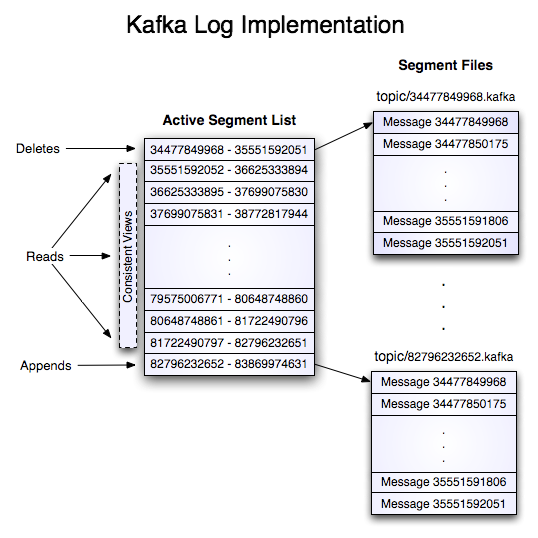
\includegraphics[scale=0.5]{5}
 	\caption{Data inside a Kafka Queueing Server, from \citep{kreps2011kafka}}
 	\label{fig:gdull05}
 \end{figure}



Another interesting use of Log Structured Storage is in "Log-structured merge-tree". LSM trees allow high write rates due to the data being stored in a log structured format first and then being written to a tree like structure \citep{o1996log}.

\subsection{Memory Reliability }

Reliability of memory is important in any computing system. The data in the memory can either be corrected or reverted back to its previous state. To revert or fix an error, the error must first be detected.

\subsubsection{Memory Reliability Techniques}
	There are many error detection techniques,one of the simplest is to use a parity bit wherein the number of bits are counted whose value is 1, if the count is odd then the parity bit is set to 1 and if the count is even, the parity bit is set to 0. During the check, the bits are counted again and the new parity is matched against the existing parity bit \citep{b1x}.\\
	
	Another important technique is the use of hamming code which can detect errors which are up to a length of 2 bits \citep{moon2005error}. But this does not work with larger data sets and the only way out is to undo the corrupt data to the previous one so that the system can still go on running. One way of reverting to the previous state is by using Memory Interleaving\citep{burnett1970study}.	
	
\subsubsection{Reliability with Memory Interleaving}


Memory Interleaving was brought in for to minimize the effects of slow RAM speeds, but it can also be used to increase the reliability of memory \citep{burnett1970study}.\\

\begin{table}[!htb]
	\centering
	\caption{Non Interleaved Memory}
	\label{table:mylabel}
	\begin{tabular}{l}
		\hline
		\multicolumn{1}{|l|}{0000 0001}                   \\ \hline
		\multicolumn{1}{|l|}{0000 0010}                   \\ \hline
		\multicolumn{1}{|l|}{0000 0011}                   \\ \hline
		\multicolumn{1}{|l|}{0000 0100}                   \\ \hline
		\multicolumn{1}{|l|}{0000 0101}                   \\ \hline
		\multicolumn{1}{|l|}{0000 0110}                   \\ \hline
		\multicolumn{1}{|l|}{0000 0111}                   \\ \hline
                                
	\end{tabular}
\end{table}

Table \ref{table:mylabel} shows memory when it is not interleaved. Data is stored in the same bank or module. If any error occurs it simply cannot be restored to a previous state.\\

\begin{table}[!htb]
	\centering
	\caption{Interleaved Memory}
	\label{table:mylabel2}
	\begin{tabular}{|l|l|}
		\hline
		0000 0000 & 0000 0001 \\ \hline
		0000 0010 & 0000 0011        \\ \hline
		0000 0100 & 0000 0101       \\ \hline
		0000 0110 & 0000 0111       \\ \hline
	
	\end{tabular}
\end{table}

Table \ref{table:mylabel2} shows memory when it is interleaved using 2 banks. Data is stored in the even and odd banks. If the data is even it is stored in the even bank and if the data is odd it is stored in the odd bank. If any error occurs in one bank, the data from the other bank is used. 

\subsection{Interleaving Applications}
Disk Interleaving is one of the primary examples of interleaving \citep{kim1986synchronized0} \citep{kim1991asynchronous} wherein interleaving is used for increasing the speed of data access from multiple disks and for error correction. This proposal uses interleaving to get rid of the WAL(Write Ahead Log) which is used for undoing a transaction\citep{mohan1992aries}.


\section{Research Method and Specification}



\subsection{Analysis of existing systems}

There are a handful of queueing servers available to be used. Few of these servers are open source and have the necessary components required for the analysis. The analysis will be based on the following

\begin{description}
	\item [Clustering Approach:] 
	The queueing system will be analysed to see if they support clustering in the first place. if they support clustering, what kind of clustering do they support - fully mirrored or sharded. This is important as benchmarks may differ based on different clustering techniques. Clustering also defines how the queueing system scales \citep{cattell2011scalable} and benchmark tests may have to be tweaked accordingly.
	\item [Data Location:]
	The queueing system will be analysed to see where it stores the data. The data can be stored either in entirely in primary memory or entirely in the secondary memory such as a disk. It can be a combination of both to improve speeds as most modern queuing servers do.
	\item [Logical Abstraction:]
	The queueing system can sometimes abstract multiple queues as one. They also have features where one queue can export data to multiple queues. This is checked so that performance benchmarks tests can take into consideration the use of multiple queues. 
	
\end{description}


\subsection{Performance Benchmark Analysis}

Performance Benchmark tests are done so as to see how existing queueing servers perform under various conditions.

\begin{description}
	\item [Enqueueing Benchmark:] 
	The queueing system will be benchmarked to see how the queue performs based on the number of operations per second. The number of queues will be increased to see how it affects the write operations.
	
	\item [Dequeueing Benchmark:]
	Dequeueing involves both read and write operations as data once read will have to be deleted from the queue as well. The queueing system will be benchmarked to see how the queue performs based on the number of dequeue operations per second. Similar to the enqueueing test, the number of queues will be increased to see how it affects the write operations.
	
	\item [Queue Creation and Deletion Benchmark:]
	The queueing systems can create and delete queues at a certain rate. This rate of creation and deletion will be benchmarked. This is required as the proposal has an entirely new way of creating a queue and this will inevitably affect the time for creation and deletion. 
	
\end{description}


\subsection{Design Goals and Decisions}

  \begin{figure}[!htb]
  	\centering
  	\textbf{}\par\medskip
  	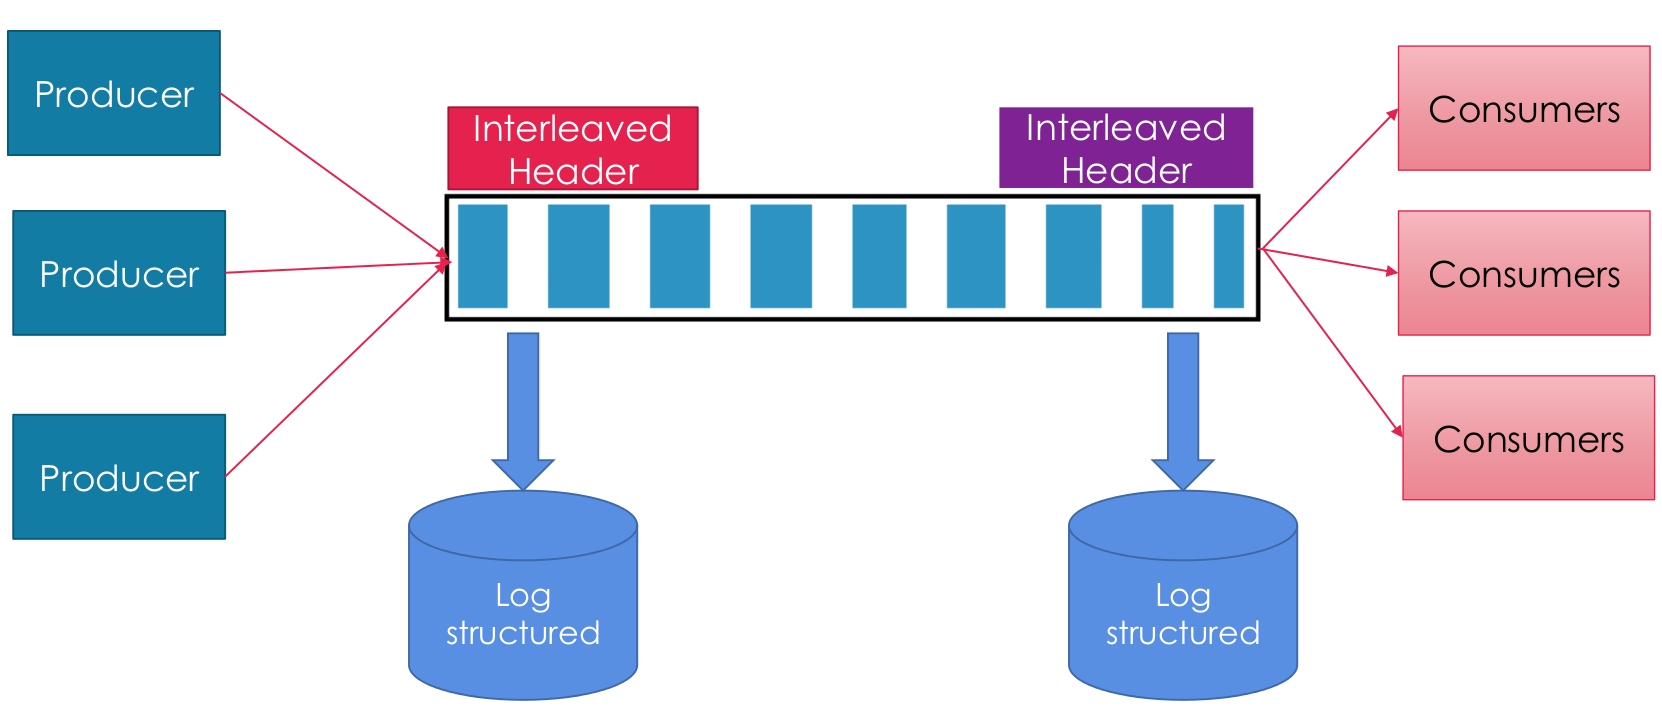
\includegraphics[scale=0.3]{8}
  	\caption{Log Structure Data Element Specification}
  	\label{fig:gdull08}
  \end{figure} 
  
Figure \ref{fig:gdull08} shows the design of the new architure for a durable queue. The goals that must be achieved using the proposed design are as follows:

\begin{enumerate}
	\item A queue for large data (grow till the disk is full).
	\item Must be fast.
	\begin{itemize}
		\item Constant performance O(1) irrespective of the size of the queue.
		\item Must allow Parallel Push and Pop operations. 
	\end{itemize}
	\item Durable.
	\begin{itemize}
		\item Must realize when the metadata pointers are corrupted.
		\item Must be capable of doing a rollback using the metadata. 
		\item If required, Rollback even without the metadata file.
	\end{itemize}
	\item Space recovery without pause
\end{enumerate}

  
  
  \subsubsection{Header Design}
  One of the important design decisions is how a header can be refactored to have multiple processes access it and also include the feature of memory interleaving within it \citep{burnett1970study}.
 
  \begin{figure}[!htb]
  	\centering
  	\textbf{}\par\medskip
  	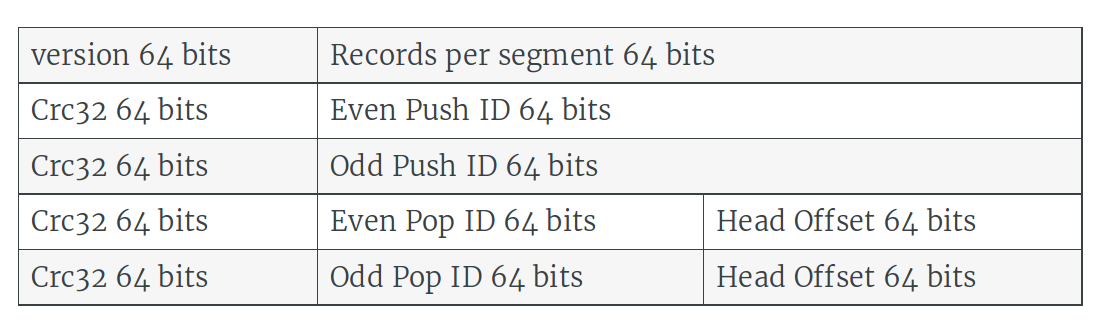
\includegraphics[scale=0.4]{6}
  	\caption{Interleaved Header Structure}
  	\label{fig:gdull06}
  \end{figure}
  
As shown in figure \ref{fig:gdull06}, there are two blocks (for Push: rows 2 and 3 and for Pop: rows 4 and 5). The push block is utilized by a process that enqueues data into the queue while the pop block is used by a process dequeuing data out of the queue. ID will go on incrementing both for push and pop independent of each other.

\begin{enumerate}
	\item The Crc32 for a row in the push block is the checksum of Push Id.
	\item The Crc32 for a row in the pop block is the checksum of Pop Id and Head Offset.
\end{enumerate}



The central idea here is to roll back. It is known that although disk access can be random, the actual write operation is still linear. The proposed design takes advantage of this to be certain that at any given time only one section, either even or odd block can get corrupted due to failure.

 \subsubsection{Log Structure Specifications}
 
 
  \begin{figure}[!htb]
  	\centering
  	\textbf{}\par\medskip
  	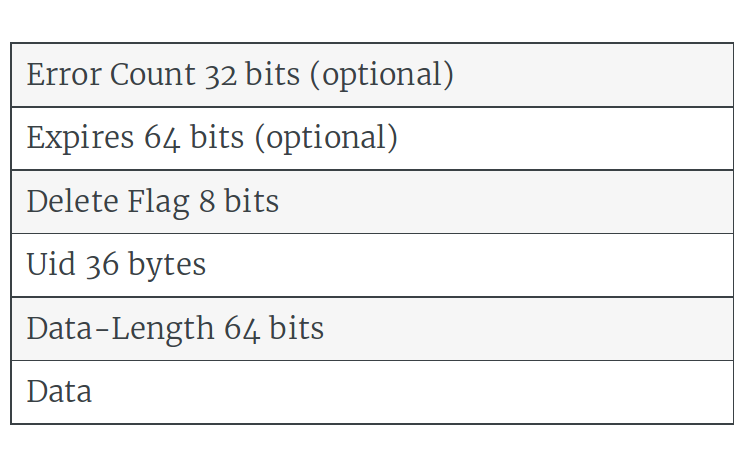
\includegraphics[scale=0.4]{7}
  	\caption{Log Structure Data Element Specification}
  	\label{fig:gdull07}
  \end{figure}
  
 Figure \ref{fig:gdull07} shows the Log Structure specification for the data element, It basically consists of 6 fields.
  
\begin{description}
    \item [Error Count:] 
    The Error Count is a count that holds the number of errors that a data element has gone through. for example, if a node picks the data item and there was an error while processing. The node sends an acknowledgement specifying the error. The queueing server will re-queue the item and increment its error count.
    
    \item [Expires:]
    Some data elements on the queue can be expirable, for example, if the task is to send emails to people on a particular day and the day has passed. The elements which have those tasks will be deleted from the queue by the server. The Expires property stores the expiry timestamp for this purpose.
    
    \item [Delete Flag:]
    The Delete Flag is used for marking an item as deleted on the queue. Since this is a log structured system, There may be instances the same data may be read after recovering from a system crash. The delete flag ensures that the same data is not read again.
    
    \item [Unique ID:]
    The Unique ID is used for uniquely representing a data element on the queue. It is used by the client to send positive or negative acknowledgements against a given UID. 
	
	 \item [Data Length:]
	The Data length field gives the length of the next field, that is the data field. The data field is of variable length and it is required to store the length of the data.
	
	 \item [Data:]
	 This the actual data that will be stored. It has no particular format. It is stored directly as bytes. The client is responsible for doing the entire encoding and decoding of data.

\end{description} 

\subsubsection{Queue Operation Specifications}

\begin{description}
	\item [Creation:] 
	Create a file named Qname.meta and Qname-0.data if they do not exist.
	Fill the Qname.meta with version and records per segment from the config.
	The rest of the bytes in the meta file must be 0s and the crc32 equivalents of those zeros.
	
	\item [Opening an existing queue:]
	First step is to open the Qname.meta file, Read its contents and decide the correct state of the queue and rollback if necessary.
	
	Below is a pseudo showing the various states that a meta file block could be in. It also includes the results or the action that needs to be performed for those conditions.
	
	\begin{lstlisting}
	
 if(evenCRCValid() && evenID>oddID)
    header=even
 else if(oddCRCValid() && oddID>evenID)
    header=odd
 else if(evenCRCValid() && oddCRCValid() && evenID==oddID) 
   //Initial condition
   header=odd //so that next write starts from even
 else if(evenCRCValid)
   header=even
 else if(oddCRCValid)
   header=odd
 else
   return (Metadata corrupted)
 end
	
	\end{lstlisting}
	
	\item [Segment Selection:]
	The data for a queue is spread over multiple files. Each such file is called a segment. The older segments can be deleted when all the data from them is popped. This allows us to easily reclaim space from the disk. 
	
	\item [Push Operation:]
	\begin{equation}
	Current Segment =\frac{PushId}{RecordsPerSegment}
	\end{equation}
	
	
	For Example,\\
	1. If the PushId is 0 and records per segment is 1000, then the segment where the new record has to be pushed will be 0/1000 i.e, Qname-0.data
	
	2. If the PushId is 2500 and records per segment is 1000, then the segment where the new record has to be pushed will be 2500/1000 i.e, Qname-2.data
	
	The raw data is converted into a record as described in the record format above. The record is appended to the selected segment. If the PushId+1 is even, the even block is overwritten else the odd block is overwritten \citep{burnett1970study}.
	

	
	\item [Pop Operation Specification:]
	
		\begin{equation}
		Current Segment =\frac{PopId}{RecordsPerSegment}
		\end{equation}
		
	The segment file selection will be similar to how the selection was performed for the push operation but the 'Head offset' must be set to zero when current segment is greater than the previous segment.
	
	The 'Head offset' is used to seek the record. The record is read after selecting the right segment. The 'Head offset' is incremented. If the PopId+1 is even, the even block is overwritten else the odd block is overwritten \citep{burnett1970study}.
	
	Note: “Head offset” must be set to zero when moving to the next segment and older segments can be deleted after the process successfully moves to a new segment.
	
	\item [Deletion:]
	Delete the meta file Qname.meta and all files matching the expression Qname-*.data. This operation will remove all log files along with the meta data.
	
	\item [Roll Back Specification:]
	
	If the meta file is found to be corrupt, we can re-construct the meta file again by sequentially going through the segment files.
	Segment files are in the format Qname-0.dat Qname-1.dat and so on.
	
	\begin{itemize}
		\item Select the segment with the smallest index. for ex: Qname-0.dat
		\item Multiply this index with the "Records per segment" from the config. The result of this will be stored in the meta file in the pop block.
		\item Read the segment files starting from the smallest index.
		\item Increment the pop id and head offset when encountered with records that are marked deleted. 
		\item Continue till no new deleted records are found.
		\item Similar approach must be followed for Push block, but here stop only when no new records are found.
	\end{itemize}
	
\end{description} 
  
 
  
 \subsection{Timeline}
 
 The following gantt chart shows the number of weeks on the X-Axis and the tasks that are to be the executed on the Y-Axis.
 
 \bigskip
 \bigskip
 
 \begin{gantt}{11}{12}
 \begin{ganttitle}
 \numtitle{1}{1}{12}{1}
 \end{ganttitle}
 \ganttbar{Install Queue}{0}{0.5}
 \ganttbar{Bench. Server}{0.5}{0.5}
 \ganttbar{Develop Layer}{1}{2}
 \ganttbar{Replace Layer}{3}{1}
 \ganttbar{Re-Run Benchs.}{4}{0.5}
 \ganttbar{Compare Benchs.}{4.5}{1.5}
 \ganttbar{Bench. on VM}{6}{2}
 \ganttbar{failure simulation}{8}{2}
 \ganttbar{Compile results}{10}{1}
 \ganttbar{Finalize paper}{11}{1}
 \end{gantt}

 \bigskip
 
\begin{itemize}
	\item The first phase involves installing and configuring an open source queueing server. 
	\item After the installation, several benchmarks are run to see how the server performs in different conditions. The conditions will include different processor speeds, different number of processor cores and varying size of memory. 
	\item Then the proposed solution is developed and this solution will replace the previously benchmarked queueing server's storage layer. 
	\item After the replacement, The benchmark tests are performed again on the server that has the newly proposed solution and then the benchmarks are compared. 
	\item Then both the versions are compared based on how they perform in a virtualized environment to see if there is any difference compared to a bare metal environment. Testing on a virtual environment is important as cloud computing environments used shared disk rather than a dedicated one and hence performance may vary \citep{liu2014performance}.
	 \item To test the effectiveness of memory interleaving, hardware failure is simulated by halting the machine abruptly. 
	\item These tests along with the benchmarks results are  compiled and a final outcome is reached whether the proposed solution works as expected.
	\item The paper is finalized based on these results.
\end{itemize}

\section{Conclusion}
In a world where the amount of data is increasing at an exponential rate and where queues bear the burden of this data acting as a backbone of distributed systems, this proposal presents a novel approach to parallelizing operations on a durable queue and expecting that queues will be less of a performance bottleneck in the future. It describes how methods such as Memory Interleaving used in the world of High-Performance Computing could be used for a very different purpose of increasing the durability of a queue and how combining it with a Log Structured Storage for storing queue elements could be used to parallelize operations on a queue. It further describes the timeline,designs and specifications on how to go about implementing the proposal and it includes the methods for verification. 

% references
\bibliographystyle{dcu}
\bibliography{adsil}

\end{document}